\subsection{Performance Analysis}
\label{sec:evaluation-performance-analysis}
Let us now consider the experimental results about system performance recorded by our simulator.
In all the experiments we have considered values stated in Section~\ref{sec:performance-modeling-specification-model} with a preemption policy based on \textit{random selection}.

\subsection{Transient Analysis}
\label{sec:evaluation-transient-analysis}
First, we conduct a \textit{transient analysis} to evaluate the system stationary in order to (i) prove its convergence to a steady-state and (ii) estimate the duration of the transient period.
%
In fact, given a system that converges to stationary, the knowledge of the duration of the transient period is really important to conduct an effective performance evaluation. 
%
In particular, even if there exist techniques to reduce the impact of transitory measurements on the final insights, having an estimate for the duration of the transient period allows the analyst to focus performance evaluation on a system in its stationary conditions.

In Figures \ref{fig:evaluation-transient-analysis-throughput-1} and \ref{fig:evaluation-transient-analysis-throughput-2} we show the transient analysis for system running the Off-Loading Policy 1 and 2, respectively. 
In this experiment we focused on the global system throughput as it can be considered a good representation of the dependency of the system to its initial state.
The experiment has been conducted considering an ensemble of $5$ replications, where the $i+1$-th replication is initialized with the last seed of the $i$-th replication, so as to achieve the best decoupling between random sequences of different replications.

The results show that the system reaches the steady-state in about $ 2000$ simulated seconds, in both cases.
This result is not surprising because the presence of a stabilizing \textit{infinite-buffer centre}, i.e. the Cloud, largely compensates the possible instabilities produced by the \textit{finite-buffer centre}, i.e. the Cloudlet.

\begin{figure}
	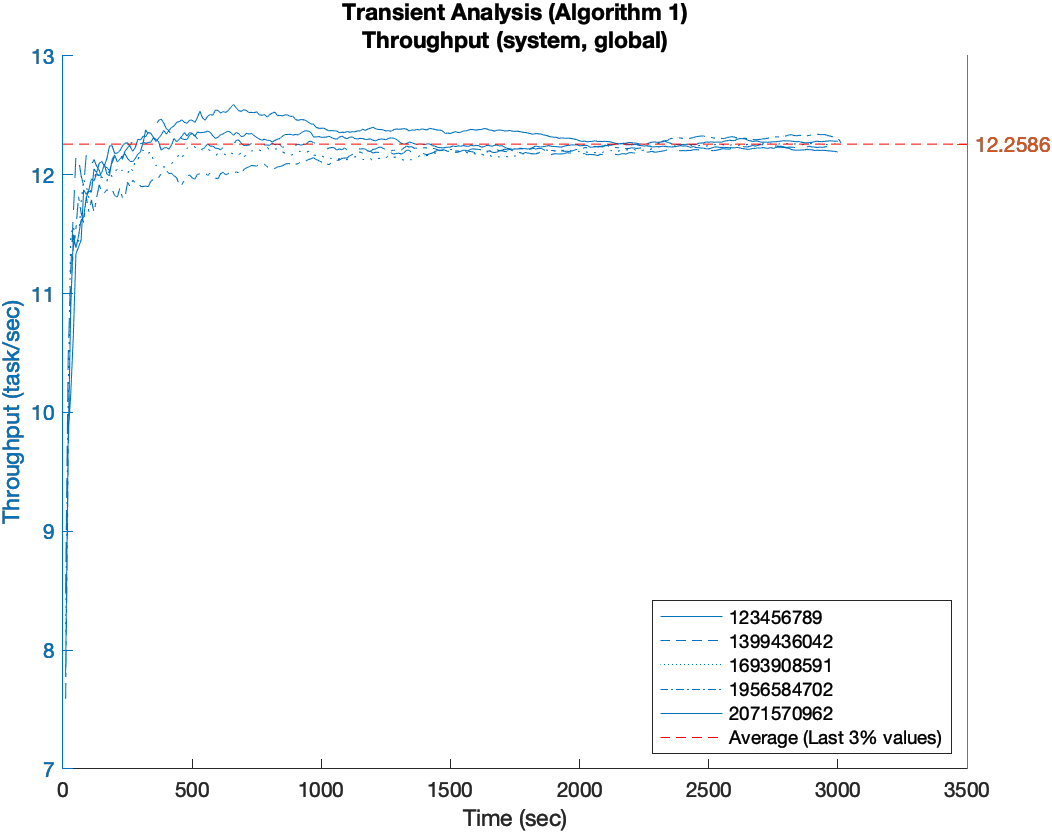
\includegraphics[width=\columnwidth]{fig/evaluation-transient-analysis-throughput-algorithm-1}
	\caption{Transient analysis for the system with OP1.}
	\label{fig:evaluation-transient-analysis-throughput-1}
\end{figure}

\begin{figure}
	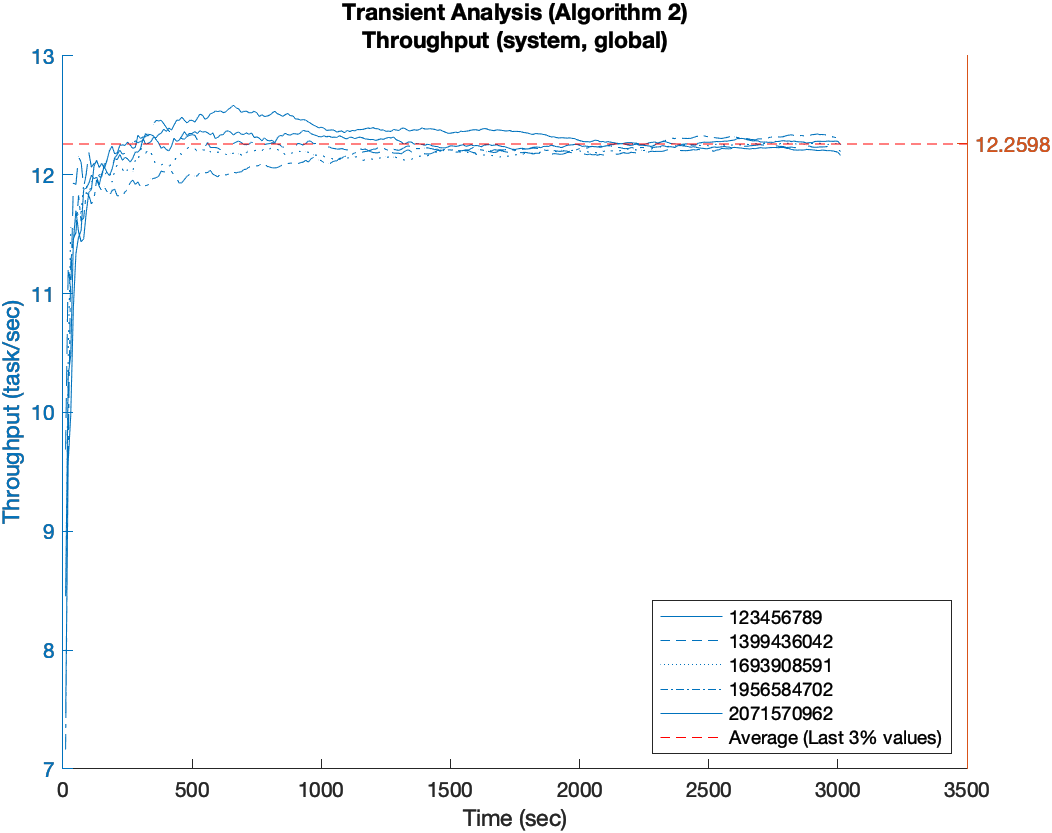
\includegraphics[width=\columnwidth]{fig/evaluation-transient-analysis-throughput-algorithm-2}
	\caption{Transient analysis for the system with OP2 (S=N=20).}
	\label{fig:evaluation-transient-analysis-throughput-2}
\end{figure}


\subsection{Steady-State Analysis}
Let us now focus on the performance evaluation in the steady-state, taking into account the following metrics:

\begin{enumerate}
	\item \textit{response time} both global and classed, both for the system as a whole and for each subsystem;
	
	\item \textit{throughput} both global and classed, both for the system as a whole and for each subsystem;
	
	\item \textit{population} both global and classed, both for the system as a whole and for each subsystem;
	
	\item \textit{interrupted ratio} for tasks belonging to the $2^{nd}$ class.	
	
	\item \textit{interrupted response time} for tasks belonging to the $2^{nd}$ class.
\end{enumerate}

In particular, it is interesting to compare performance metrics in the following scenarios:

\begin{enumerate}
	\item \textit{Off-Loading Policy 1}, where no priority distinction is made between classes of tasks;
	
	\item \textit{Off-Loading Policy 2 ($S=20$)}, where $1^{st}$ class tasks have higher priority than $2^{nd}$ class tasks and the latter have also both (i) high probability to be served by the Cloudlet and, as a consequence, (ii) high risk to be interrupted and incur in the restart overhead.
	
	\item \textit{Off-Loading Policy 2 ($S=5$)}, where $1^{st}$ class tasks have  higher priority than $2{nd}$ class tasks and the latter have also both (i) low probability to be served by the Cloudlet and, as a consequence, (ii) low risk to be interrupted and incur in the restart overhead.
\end{enumerate}

In Tables \ref{tbl:evaluation-performance-metrics-1}, \ref{tbl:evaluation-performance-metrics-2-20} and \ref{tbl:evaluation-performance-metrics-2-5}, we show the theoretical and experimental results for the system with Off-Loading Policy 1,  Off-Loading Policy 2 having $N=S=20$ and Off-Loading Policy 2 having $N=20,S=5$, respectively.

Experimental results have been computed assuming a system with $S=N=20$ and batch means computations with $k=64$ batches of dimension $b=512$ each.
%
Theoretical results have been computed using the formulas presented in Section~\ref{sec:analytical-model}.
%, assuming the routing probabilities shown in Table~\ref{tbl:evaluation-routing-probabilities} and $E[T_{clt,2,lost}]=1.47445;s$.

We attribute any gap between the theoretical and experimental results to the stringent assumptions we made on the analytical model, which can inevitably cause approximations in the final results.

By comparing the three scenarios, we conclude that:

\begin{enumerate}
	\item the introduction of OP2 w.r.t. OP1 improves the system response time for $1^{st}$ class tasks, whereas it worsen it for $2^{nd}$ class tasks. 
	This is expected because OP2 increases the probability for a $1^{st}$ class task to be served by the Cloudlet, which is faster than the Cloud.
	
	\item moving from $S=20$ to $S=5$ does not have a significant impact on response time for $1^{st}$ class tasks, whereas it improves it for $2^{nd}$ class tasks.
	This may sound less intuitive because a high $S$ increases the probability for a $2^{nd}$ class task to be served by the Cloudlet, which is faster than the Cloud. Nevertheless, a high $S$ also increases the probability for the same tasks to be interrupted in the Cloudlet and lose time.
	
	\item the previous two points suggest us that a fine tuning of $S$ together with a smarter policy for the selection of the $2^{nd}$ class tasks to interrupt, e.g. interrupt the youngest task in order to minimize the lost time in Cloudlet, would be really valuable to leverage the power of OP2 over OP1.
\end{enumerate}

%\begin{figure}
%	\begin{center}
%		\begin{tabular}{|c||c|c|}
%			\hline
%			Measure & Theoretical & Experimental\\
%			\hline
%			$a_{clt,1}$  & $0.978326334857105$ & $0.97911346521$ \\
%			$a_{clt_2}$  & $0.603529764734761$ & $0.60502880468$ \\
%			$r$          & $0.183573830264005$ & $0.15525744148$ \\	
%			\hline
%		\end{tabular}
%	\end{center}
%	\caption{Routing probabilities: comparison between the theoretical result, computed with the analytical model, and the experimental result, computed leveraging our simulator.}
%	\label{tbl:evaluation-routing-probabilities}
%\end{figure}

\begin{figure}
	\begin{center}
		\begin{tabular}{|c||c|c|}
\hline
Measure & Theoretical & Experimental \\
\hline
$N_{clt}$  & $19.0079214380542$ & $18.9657556411\pm 0.061761348$ \\ 
$N_{clt,1}$  & $6.94705758142083$ & $6.9174978557\pm 0.0221472832$ \\ 
$N_{clt,2}$  & $12.0608638566334$ & $12.0482577854\pm 0.0676551914$ \\ 
$T_{clt}$  & $2.97808012093726$ & $2.9329442796\pm 0.0299023279$ \\ 
$T_{clt,1}$  & $2.22222222222222$ & $2.1928106049\pm 0.017782072$ \\ 
$T_{clt,2}$  & $3.7037037037037$ & $3.6392880155\pm 0.0399050928$ \\ 
$X_{clt}$  & $6.38260915293038$ & $6.4226859577\pm 0.0204460156$ \\ 
$X_{clt,1}$  & $3.12617591163937$ & $3.1401150807\pm 0.0196271592$ \\ 
$X_{clt,2}$  & $3.25643324129101$ & $3.282570877\pm 0.0064520454$ \\ 
\hline 
$N_{cld}$  & $25.1024179839379$ & $24.8788290839\pm 0.4843210347$ \\ 
$N_{cld,1}$  & $11.4952963534425$ & $11.6176870943\pm 0.2291824053$ \\ 
$N_{cld,2}$  & $13.6071216304954$ & $13.2611419897\pm 0.2620827898$ \\ 
$T_{cld}$  & $4.2956713711267$ & $4.1967104264\pm 0.0414272512$ \\ 
$T_{cld,1}$  & $4.0$ & $3.965860097\pm 0.0313637462$ \\ 
$T_{cld,2}$  & $4.54545454545455$ & $4.423180833\pm 0.0515154164$ \\ 
$X_{cld}$  & $5.86739084706962$ & $5.8591880304\pm 0.1174124089$ \\ 
$X_{cld,1}$  & $2.87382408836063$ & $2.8987603707\pm 0.05909048$ \\ 
$X_{cld,2}$  & $2.99356675870899$ & $2.9604276598\pm 0.0591551518$ \\ 
\hline 
$N_{sys}$  & $43.5447719188013$ & $43.8445847251\pm 0.5448264622$ \\ 
$N_{sys,1}$  & $21.3280515520659$ & $18.53518495\pm 0.2227839341$ \\ 
$N_{sys,2}$  & $22.2167203667353$ & $25.3093997751\pm 0.3259203125$ \\ 
$T_{sys}$  & $3.85670891708856$ & $3.535972929\pm 0.0398351701$ \\ 
$T_{sys,1}$  & $2.87973287200309$ & $3.0441528892\pm 0.0334852226$ \\ 
$T_{sys,2}$  & $4.7946059203706$ & $4.0113028172\pm 0.0458354286$ \\ 
$X_{sys}$  & $12.25$ & $12.2818739881\pm 0.1031221489$ \\ 
$X_{sys,1}$  & $6.0$ & $6.0388754514\pm 0.0428513144$ \\ 
$X_{sys,2}$  & $6.25$ & $6.2429985368\pm 0.0612224429$ \\ 
\hline 
		\end{tabular}
	\end{center}
	\caption{Performance metrics with OP1.}
	\label{tbl:evaluation-performance-metrics-1}
\end{figure}

\begin{figure}
	\begin{center}
		\begin{tabular}{|c||c|c|}
\hline
Measure & Theoretical & Experimental \\
\hline
$N_{clt}$  & $18.6861348679399$ & $18.6256514408\pm 0.0664027232$ \\ 
$N_{clt,1}$  & $13.0443511314281$ & $13.0073445344\pm 0.1191309252$ \\ 
$N_{clt,2}$  & $5.64178373651183$ & $5.6183069064\pm 0.0580175732$ \\ 
$T_{clt}$  & $2.52746236202645$ & $2.486244959\pm 0.0151247853$ \\ 
$T_{clt,1}$  & $2.22222222222222$ & $2.1905842105\pm 0.0188772557$ \\ 
$T_{clt,2}$  & $3.70370370370371$ & $3.6127254526\pm 0.0218732553$ \\ 
$X_{clt}$  & $7.39323961800082$ & $7.454305304\pm 0.0138303964$ \\ 
$X_{clt,1}$  & $5.86995800914263$ & $5.9037777336\pm 0.0317748218$ \\ 
$X_{clt,2}$  & $1.52328160885819$ & $1.5505275704\pm 0.0211578776$ \\ 
\hline 
$N_{cld}$  & $23.8042750961159$ & $23.5478911244\pm 0.4188925236$ \\ 
$N_{cld,1}$  & $0.520167963429486$ & $0.6022354192\pm 0.0212165955$ \\ 
$N_{cld,2}$  & $23.2841071326864$ & $22.9456557052\pm 0.4033574016$ \\ 
$T_{cld}$  & $4.93752153860152$ & $4.8126915196\pm 0.0521333156$ \\ 
$T_{cld,1}$  & $4.0$ & $4.0785104754\pm 0.0824838383$ \\ 
$T_{cld,2}$  & $4.9584658104444$ & $4.8350983148\pm 0.0537793315$ \\ 
$X_{cld}$  & $4.85676038199918$ & $4.8308542672\pm 0.0900199085$ \\ 
$X_{cld,1}$  & $0.130041990857372$ & $0.1461573408\pm 0.0056344117$ \\ 
$X_{cld,2}$  & $4.72671839114181$ & $4.6846969265\pm 0.0850510603$ \\ 
\hline 
$N_{sys}$  & $37.3687941909734$ & $42.1735425651\pm 0.4841637065$ \\ 
$N_{sys,1}$  & $18.3030828690482$ & $13.6095799536\pm 0.1357291534$ \\ 
$N_{sys,2}$  & $19.0657113219252$ & $28.5639626116\pm 0.3531052396$ \\ 
$T_{sys}$  & $4.48013019690776$ & $3.4029598386\pm 0.0341771009$ \\ 
$T_{sys,1}$  & $1.69742545748866$ & $2.2364277477\pm 0.019497486$ \\ 
$T_{sys,2}$  & $7.15152674675009$ & $4.5340442283\pm 0.0450395882$ \\ 
$X_{sys}$  & $12.25$ & $12.2851595712\pm 0.1020002877$ \\ 
$X_{sys,1}$  & $6.0$ & $6.0499350743\pm 0.0368009794$ \\ 
$X_{sys,2}$  & $6.25$ & $6.2352244969\pm 0.0666726067$ \\ 
\hline
\hline
		\end{tabular}
	\end{center}
	\caption{Performance metrics with OP2 (N=S=20).}
	\label{tbl:evaluation-performance-metrics-2-20}
\end{figure}

\begin{figure}
	\begin{center}
		\begin{tabular}{|c||c|c|}
\hline
Measure & Theoretical & Experimental \\
\hline
$N_{clt}$  & $13.0466462362487$ & $13.0433572946\pm 0.1000197871$ \\ 
$N_{clt,1}$  & $13.0443511314281$ & $13.0404451177\pm 0.100159524$ \\ 
$N_{clt,2}$  & $0.00229510482068997$ & $0.0029121769\pm 0.0003746161$ \\ 
$T_{clt}$  & $2.22237860239078$ & $2.1917257858\pm 0.0163608319$ \\ 
$T_{clt,1}$  & $2.22222222222222$ & $2.192336913\pm 0.0157853478$ \\ 
$T_{clt,2}$  & $3.7037037037037$ & $1.8386687645\pm 0.2026686866$ \\ 
$X_{clt}$  & $5.87057768744421$ & $5.9175159391\pm 0.0300427259$ \\ 
$X_{clt,1}$  & $5.86995800914263$ & $5.914127608\pm 0.032255318$ \\ 
$X_{clt,2}$  & $0.000619678301586293$ & $0.0033883312\pm 0.0024619263$ \\ 
\hline 
$N_{cld}$  & $28.9336326367421$ & $28.7592002142\pm 0.3244410982$ \\ 
$N_{cld,1}$  & $0.520167963429492$ & $0.5587933651\pm 0.025284303$ \\ 
$N_{cld,2}$  & $28.4134646733126$ & $28.2004068491\pm 0.3046711815$ \\ 
$T_{cld}$  & $4.53697681371044$ & $4.4634171571\pm 0.0415547819$ \\ 
$T_{cld,1}$  & $4.0$ & $4.0717091521\pm 0.1405913069$ \\ 
$T_{cld,2}$  & $4.54680729861638$ & $4.4716070089\pm 0.0421282903$ \\ 
$X_{cld}$  & $6.37942231255579$ & $6.3677605014\pm 0.0759473595$ \\ 
$X_{cld,1}$  & $0.130041990857373$ & $0.1355383067\pm 0.0066949314$ \\ 
$X_{cld,2}$  & $6.24938032169841$ & $6.2322221947\pm 0.070364113$ \\ 
\hline 
$N_{sys}$  & $42.4981517315996$ & $41.8025575089\pm 0.4144222505$ \\ 
$N_{sys,1}$  & $20.8154212562937$ & $13.5992384828\pm 0.1218741864$ \\ 
$N_{sys,2}$  & $21.6827304753059$ & $28.203319026\pm 0.3045407478$ \\ 
$T_{sys}$  & $3.77115618506066$ & $3.3697751086\pm 0.031978144$ \\ 
$T_{sys,1}$  & $1.49255296973888$ & $2.2347925896\pm 0.0172187976$ \\ 
$T_{sys,2}$  & $5.95861527176956$ & $4.4699170668\pm 0.0432799606$ \\ 
$X_{sys}$  & $12.25$ & $12.2852764406\pm 0.104073231$ \\ 
$X_{sys,1}$  & $6.0$ & $6.0496659147\pm 0.037506365$ \\ 
$X_{sys,2}$  & $6.25$ & $6.2356105259\pm 0.0679721177$ \\ 
\hline 
		\end{tabular}
	\end{center}
	\caption{Performance metrics with OP2 (N=20,S=5).}
	\label{tbl:evaluation-performance-metrics-2-5}
\end{figure}

%%
% DISTRIBUTION ANALYSIS
%%
%\subsection{Distribution Analysis}
%\label{sec:evaluation-distribution-analysis}
%In this Section we show the distribution analysis of the Cloudlet global throughput. 
%In particular, we focus on both (i) the Probability Density Function (PDF) estimation leveraging distribution fitting, and (ii) the comparison between theoretical and experimental Cumulative Distribution Function (CDF).

%In Figure~\ref{fig:evaluation-distribution-analysis-pdf-throughput-cloudlet-global} and  Figure~\ref{fig:evaluation-distribution-analysis-cdf-throughput-cloudlet-global} we show the PDF estimation and the CDF analysis, respectively, for the global Cloudlet throughput when $S=N=20$, where we adopted the \textit{Freedman-Diaconis Rule} for the binning schema.
%Results show that the best fitting is the \textit{Normal Distribution} with parameters $\mu\approx7.403$ and $\sigma\approx0.364$.
%
%The Normal behavior shown here can be considered as a further good proof of both the system stationary and the effectiveness of the batch means as a tool to study steady-state statistics.

%\begin{figure}
%	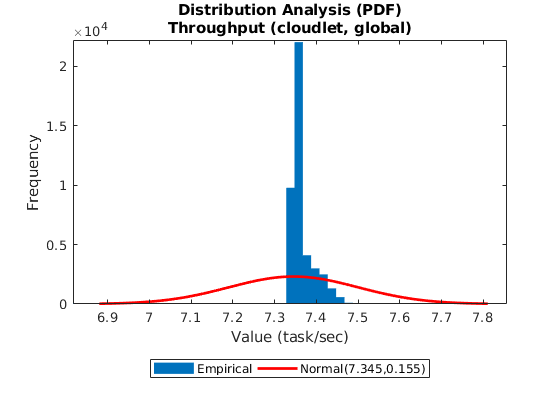
\includegraphics[width=\columnwidth]{fig/evaluation-distribution-analysis-pdf-throughput-cloudlet-global}
%	\caption{Distribution analysis (Probability Distribution Function)for the Cloudlet global throughput with threshold $S=N=20$.}
%	\label{fig:evaluation-distribution-analysis-pdf-throughput-cloudlet-global}
%\end{figure}

%\begin{figure}
%	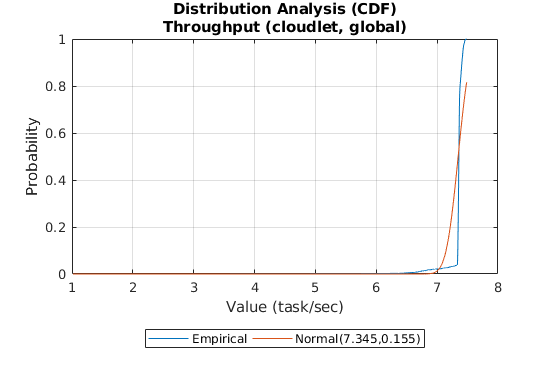
\includegraphics[width=\columnwidth]{fig/evaluation-distribution-analysis-cdf-throughput-cloudlet-global}
%	\caption{Distribution analysis (Cumulative Distribution Function) for the Cloudlet global throughput with threshold $S=N=20$.}
%	\label{fig:evaluation-distribution-analysis-cdf-throughput-cloudlet-global}
%\end{figure}